\section{Motivation}\label{sec:motivation}

% Overview

To use stream ciphers for performant FDE, StrongBox leverages two key insights:
1) the overwrite-averse \emph{append-mostly} behavior of Log-structured File
Systems (LFS) and 2) the division of the backing store into discrete same-size
metadata-managed units \emph{above the block I/O layer} referred to as
\emph{nuggets}. When the rare overwrite does occur during I/O, StrongBox
modifies the cipher keystream or \emph{rekeys} the affected nugget(s) to prevent
a confidentiality violation.

This approach naturally leads to transitioning individual nuggets between any
cipher during runtime. This is because 1) encryption and decryption of nuggets
is compartmentalized; nugget-level operations occur independently of one another
and 2) all rekeying operations end up committing data to "empty"
(\ie{initialized with random data}) space on the backing store.

We can build on this behavior by abstracting the rekeying process out into a
\emph{re-ciphering} process, whereby the key \emph{and the cipher used to
encrypt/decrypt the nugget} can both be switched at runtime. This allows us to
trade off between different ciphers and their characteristics dynamically,
whereas prior work can only accomplish a static tradeoff at compile time or
filesystem initialization.

\subsection{Quantifying the Security Dimension}

To reason about trading off the security guarantees provided by various ciphers,
the strength of these guarantees must be quantified through scoring. For our
purposes, we arrived at three key features that, when scored, give us a useful
quantification of cipher security (see: \tblref{security-quant}).

\begin{itemize}

 \item \emph{Output randomization.} A cipher that exhibits output randomization
 can output ciphertext non-deterministically given the same input, which is
 extremely useful for FDE\@. This is a binary feature in that a cipher either
 outputs deterministically or it does not. A cipher with output randomization
 scores a 1 for this feature while a cipher without it scores a 0.

 \item \emph{Resistance to cryptanalysis.} A cipher that is resistant to
 cryptanalysis can resist theoretical cryptanalytical attacks such as
 known-plaintext and chosen-plaintext attacks, offline key-guessing attacks, et
 cetera. Scores for this feature range from 0 to 1, where 0.5 represents
 standard resistance to cryptanalysis for stream ciphers in the general case\@.

 \item \emph{Round count vs standard.} The ciphers we examine in this research
 are all constructed around the notion of \emph{rounds}, where a higher number
 of rounds implies a stronger confidentiality guarantee. This feature represents
 how many rounds the cipher executes compared to the accepted "standard" round
 count for that cipher. For instance, ChaCha8 is a reduced round version of the
 standard ChaCha20. Variants are distributed evenly from 0-1. For instance,
 ChaCha8 scores 0, ChaCha12 scores 0.5, and ChaCha20 scores 1\@.

\end{itemize}

\begin{table}[]
   \begin{tabular}{@{}lllll@{}}
   \toprule
   \textbf{Cipher} & \textbf{OR} & \textbf{CR} & \textbf{RR/RK} & \textbf{Rank} \\ \midrule
   ChaCha8         & 0           & 0.5         & 0              & 0.5           \\
   ChaCha12        & 0           & 0.5         & 0.5            & 1             \\
   ChaCha20        & 0           & 0.5         & 1              & 1.5           \\
   Salsa8          & 0           & 0.4         & 0              & 0.4           \\
   Salsa12         & 0           & 0.4         & 0.5            & 0.9           \\
   Salsa20         & 0           & 0.4         & 1              & 1.4           \\
   AES128-CTR      & 0           & 0.5         & 0              & 0.5           \\
   AES256-CTR      & 0           & 0.5         & 1              & 1.5           \\
   HC128           & 0           & 0.5         & 0              & 0.5           \\
   HC256           & 0           & 0.5         & 1              & 1.5           \\
   Rabbit          & 0           & 0.4         & 1              & 1.4           \\
   Sosemanuk       & 0           & 0.4         & 1              & 1.4           \\
   Freestyle (F)   & 1           & 1           & 0              & 2             \\
   Freestyle (B)   & 1           & 1           & 0.5            & 2.5           \\
   Freestyle (S)   & 1           & 1           & 1              & 3             \\
   AES128-XTS      & 0.2         & 0.5         & 1              & 1.7
   \end{tabular}
   \caption{\TODO{Table caption goes here.}}
   \label{tbl:security-quant}
\end{table}

\subsection{Statically Trading off Energy/Latency for Security}

\begin{figure}[ht]
 \centering
  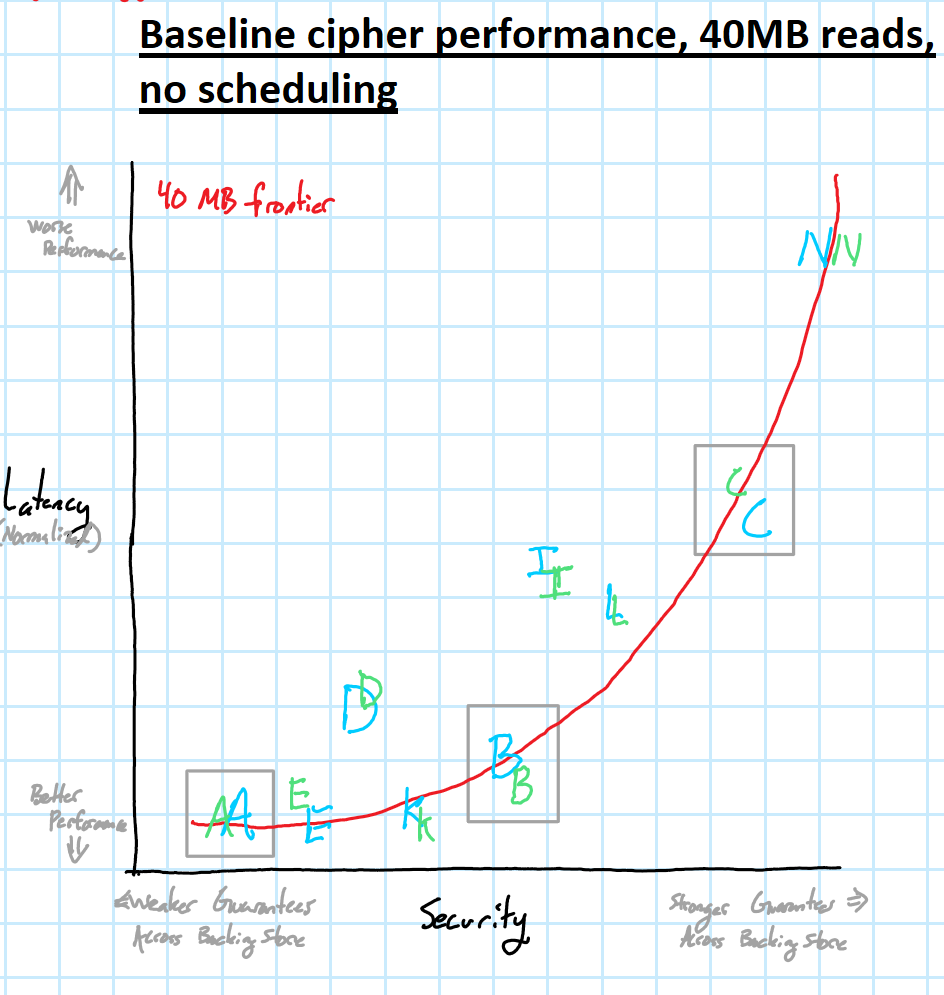
\includegraphics[width=0.8\linewidth]{drawn/1.png}
   \caption{\TODO{Caption goes here}\TODO{No curve in this version!}}\label{fig:40mb-read-frontier}
\end{figure}

\figref{40mb-read-frontier} shows the security versus I/O latency static
tradeoff between different stream ciphers under StrongBox when completing a 40MB
read of encrypted storage. The experiment was performed on an ARM big.LITTLE
Exynos Octa processor, which is similar to the processors used in the Samsung
Galaxy line of phones and other devices. \TODO{In the LaTeX figure, parateo
frontier is X while other results are some other shape. Explain this here.}

Ciphers with relatively stronger security guarantees result in higher latency
for I/O operations while ciphers with relatively weaker security guarantees
result in lower latency.

\begin{figure}[ht]
 \centering
  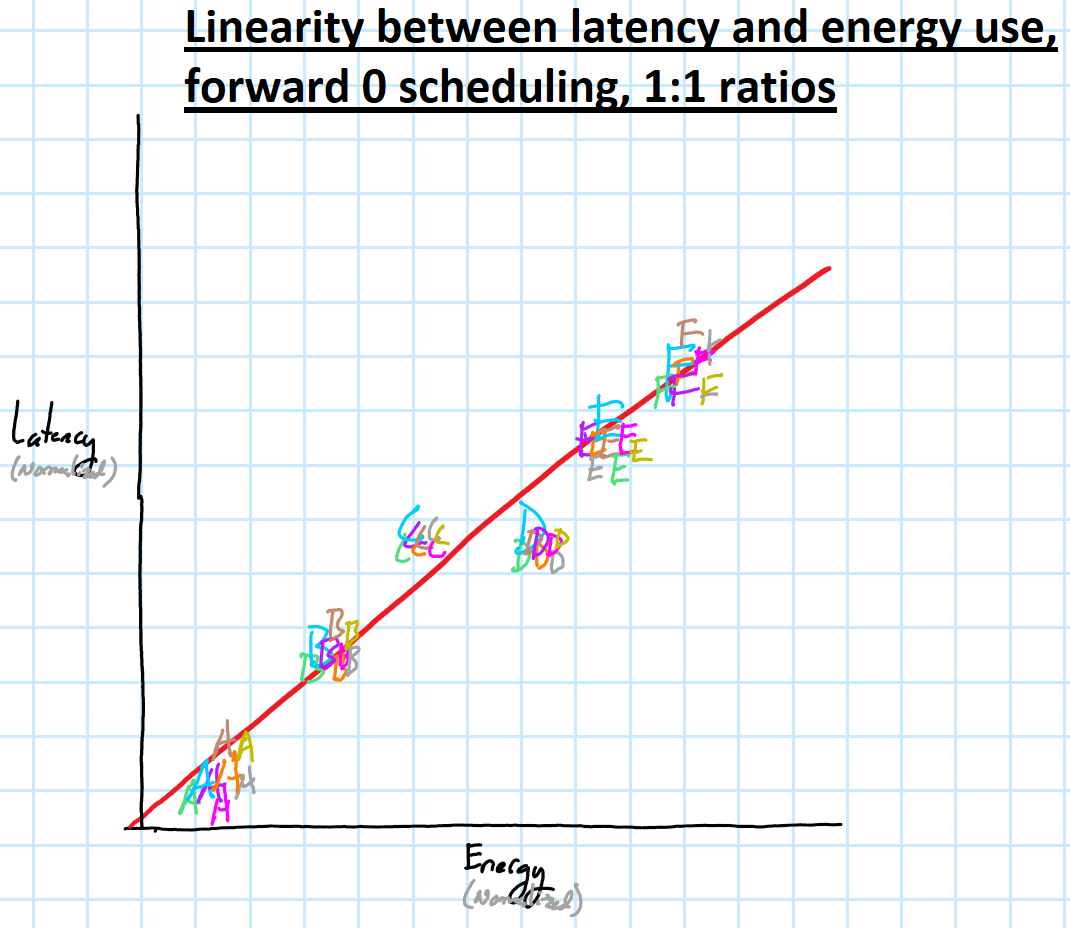
\includegraphics[width=0.8\linewidth]{drawn/5.png}
   \caption{\TODO{Caption goes here}}\label{fig:energy-latency-linearity}
\end{figure}

\figref{energy-latency-linearity} shows that, for the stream ciphers included in
our experiments, there is a linear relationship between cipher performance and
total energy used during the I/O operation.

With prior work, \TODO{we could cite other filesystems and storage layers here
other than just StrongBox, such as ZFS, dmcrypt?} cipher configuration is made
statically at compile time or at filesystem initialization. This forces
developers and end-users to choose a configuration that works best in the most
general case and stick with it, even if a different configuration becomes more
optimal at a later point. The only way to switch ciphers when a new
configuration becomes more optimal is to remake the entire filesystem.
\TODO{This paragraph should be fleshed out more?}

\subsection{Dynamically Trading off Energy/Latency for Security}

For example:\\

\noindent
\textbf{Streaming video to networked devices with a curtailed energy budget}

Text.\\

\noindent
\textbf{Massive multi-cipher document with variable security regions}

Text.
